
\subsection{Cloud Service}\label{subsec:cloud-service}

\subsubsection{Architektur}

\subsubsection*{Überblick}

Der Cloud Service wird in die zwei Domänen Notification und Configuration aufgeteilt.
Dabei ist die Domäne Notification für das Versenden von Benachrichtigungen zuständig.
Die Domäne Configuration ist für die Verwaltung der Konfigurationen und Subscriptions verantwortlich.
Die Domäne Notification benötigt zum Versenden von Benachrichtigungen Informationen, die aus der Domäne Configuration stammen.
Grundsätzlich braucht sie dazu aber nur ein kleines Subset dieser Informationen.
Sobald identifiziert ist, an wen eine Benachrichtigung gesendet werden soll und wie dieser Client erreicht werden kann, funktioniert das Versenden der Benachrichtigung komplett unabhängig von der Domäne Configuration.

Da die beiden Domänen nicht eng gekoppelt sind, wäre es denkbar die Domänenspezifische Logik in zwei separate Microservices aufzuteilen.
Die Aufteilung auf mehrere Microservices macht das System als ganzes aber direkt komplizierter.
Insbesondere Betrieb und Entwicklung wird aufwändiger, da diese Arbeiten nun über mehrere Applikationen verteilt sind.
Für den Umfang dieser Arbeit wird deshalb darauf verzichtet, den Cloud Service als echtes Micro Service System umzusetzen.
Der Cloud Service wird in als eine einzelne Spring Boot Applikation umgesetzt.
Innerhalb dieser Applikation sollen die Domänen Configuration und Notification wo immer mit vertretbarem Aufwand möchlich, getrennt bleiben.
Abhängigkeiten zwischen den beiden Domänen sind zu vermeiden.
An den Stellen wo Informationen aus der anderen Domäne nötig sind, sollen diese über ein Rest Interface abgefragt werden.
So kann die Applikation in Zukunft einfach und auf die tatsächlichen Bedürfnisse zugeschnitten in mehrere Microservices aufgeteilt werden.

\clearpage

\subsubsection*{Service Architektur}

Der Cloud Service wird nach dem Prinzip von Onion Architecture / Clean Architecture aufgebaut.

\begin{figure}[h]
    \centering
    \begin{minipage}[b]{0.5\textwidth}
        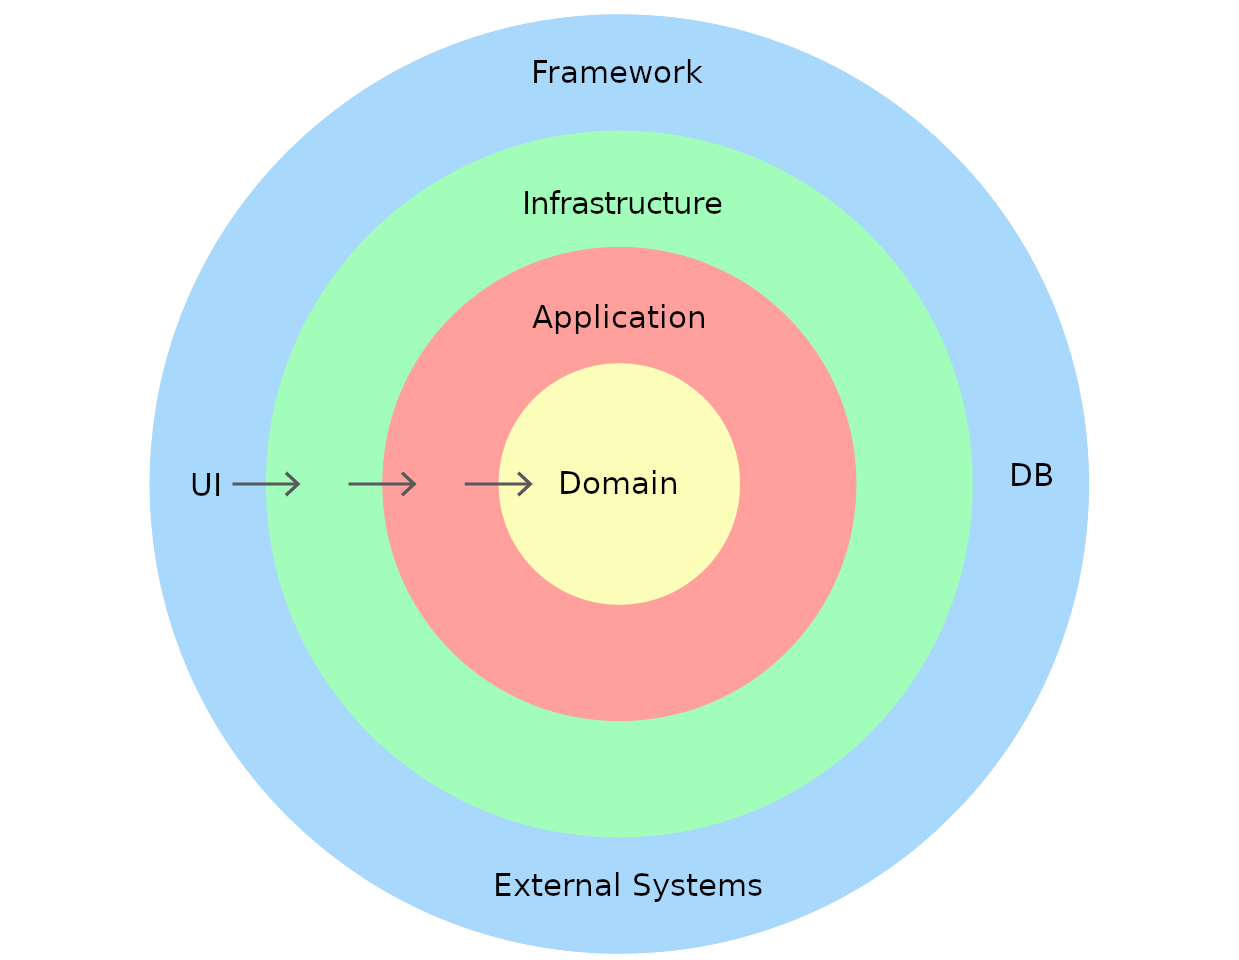
\includegraphics[width=\textwidth]{graphics/clean-architecture}
        \caption{Clean Architecture}
    \end{minipage}
\end{figure}

In Onion Architecture wird die Applikation in Layern von der Domäne im Zentrum bis hin zur Infrastruktur an den äusseren Enden definiert.
Im Wesentlichen gibt es die folgenden Layers\cite{medium-onion}.

\textbf{Domain Model}
Im Zentrum des Modells steht die Domain selbst.
Der Domain Layer darf nur Dependencies auf sich selbst haben.
Abhängigkeiten aus anderen Layers sind um jeden Preis zu vermeiden.
Abhängigkeiten aus äusseren Layer auf den Domain Layer sind hingegen immer erlaubt.

\textbf{Domain Services}
Bieten die fachliche Logik und Verhaltensweise des Domain Model Layers an.

\textbf{Application Services}
Bildet die Brücke zwischen externer Infrastruktur und den DomainServices.
Dies beinhaltet Repository Services und Rest Controllers.

\textbf{Infrastructure}
Veranschaulicht die Infrastruktur ausserhalb des Systems.
Dies beinhaltet unter anderem Datenbanken, Messaging Services und Applikationen die auf Web APIs welche der Applikation zugreifen.

\clearpage

\subsubsection*{Package Struktur}

Der Cloud Service definiert die folgenden top level Packages:

\begin{figure}[h]
    \centering
    \begin{minipage}[b]{0.9\textwidth}

        \dirtree{%
        .1 ch.fhnw.ip5.praxiscloudservice.
        .2 api.
        .2 config.
        .2 domain.
        .2 persistence.
        .2 service.
        .2 web.
    }
    \caption{Package Struktur Cloud Service}\label{fig:packagescloudservice}
    \end{minipage}
\end{figure}

\\ \\

Im Zentrum steht das Package \textbf{domain}.
Es beinhaltet alle Domänenobjekte und stellt damit alleine den Domain Layer dar.

Das Package \textbf{api} definiert Interfaces für sämtliche Domain Services.
Es beinhaltet weiter Data Transition Objects (DTOs), welche verwendet werden um Daten ausserhalb der Domain (UI oder andere Domain) abzubilden.
Es beinhaltet zudem Exceptions welche für den Cloud Service definiert werden.

Das Package \textbf{persistence} beinhaltet Services welche für Interaktion mit der Datenbank verwendet werden und  gehört zum Application Services Layer.

Das Package \textbf{service} beinhaltet die Services welche das Verhalten der Applikation modellieren und entspricht dem Domain Service Layer.

Das Package \textbf{web} beinhaltet die Controller welche REST Endpoints anbieten, sowie Clients die verwendet werden um andere REST Endpoints zu konsumieren.
Es gehört zum Application Services Layer.

Das Package \textbf{config} beinhaltet technische Konfiguration der Applikation.


\clearpage

\subsubsection{Domänenmodell}

Wie in Kapitel 4.3.1 beschrieben, teilt sich der Cloud Service in die zwei Domänenbereiche Notification und Configuration auf.
Im Folgenden wird detailliert beschrieben, wie diese Domänen aufgebaut sind.

\subsubsection*{Domäne Configuration}

\begin{figure}[h]
    \centering
    \begin{minipage}[b]{0.9\textwidth}
        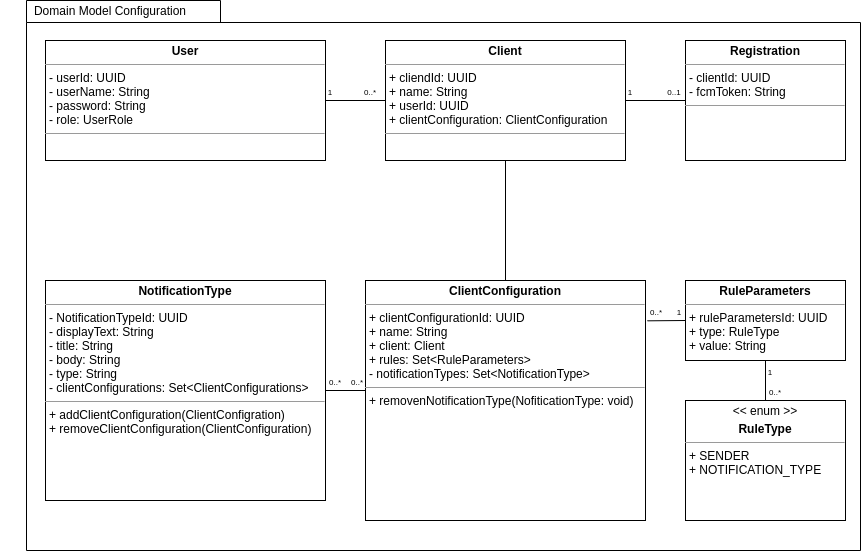
\includegraphics[width=\textwidth]{graphics/Class_Configuration_Domain}
        \caption{Domänenmodell Configuration}
    \end{minipage}
\end{figure}

\textbf{PraxisUser}
Ein Benutzer für das Praxisrufsystem.
Jeder Benutzer kann entweder die Rolel Admin oder User haben.
Admin ist für Admin UI (Praxisverantwortlicher).
User ist für Mobile Client (Praxismitarbeiter) Nutzer.

\textbf{Client}
Ein Client repräsentiert ein Gerät auf welchem der Mobile Client läuft.

\textbf{Registration}
Die Registrierung eines Clients beinhaltet die Informationen die vom Messaging Service verwendet werden können um diesem spezifischen Client eine Benachrichtigung zu stellen.
Ein Client kann nie mehrere Registrierungen haben.

\textbf{ClientConfiguration}
Stellt die Konfiguration eines Clients dar.
Die Beziehung von Client zu ClientConfiguration ist immer 1:1.
Client und ClientConfiguration sind getrennt, damit Clients auch ohne Configuration erfasst werden können.
So kann der Administrator die Geräte die er hat von Anfang an erfassen aber ers nach und nach die Konfigurationen dazu erstellen.

\textbf{NotificationType}
Der NotificationType ist die Grundlage für Notifications die versendet werden.
Der NotificationType definiert Informationen für den Inhalt von Benachrichtigungen die versendet werden.
Er beinhaltet weiter Schlüssel für Texte die in einem Client angezeigt werden können.

\textbf{RuleParameters}
RuleParameters sind die parameterisierten Werte für eine Regel.
Sie werden pro ClientConfiguration erfasst.
Sie werden von der RulesEngine ausgewertet um zu identifizieren ob ein Client sich für eine gegebene Benachrichtigung interessiert.

\textbf{RuleType}
Der RuleType bestimmt wie die Parameter für eine Regel (siehe RulePrameters) ausgewertet werden.
Für jeden Eintrag in der Tabelle RuleType muss es eine Implementierung des Interfaces RuleEvaluator geben, welche die RulesParameter Werte für den Regeltyp auswerten kann.

\subsubsection*{Configuration Services}

\begin{figure}[h]
    \centering
    \begin{minipage}[b]{0.9\textwidth}
        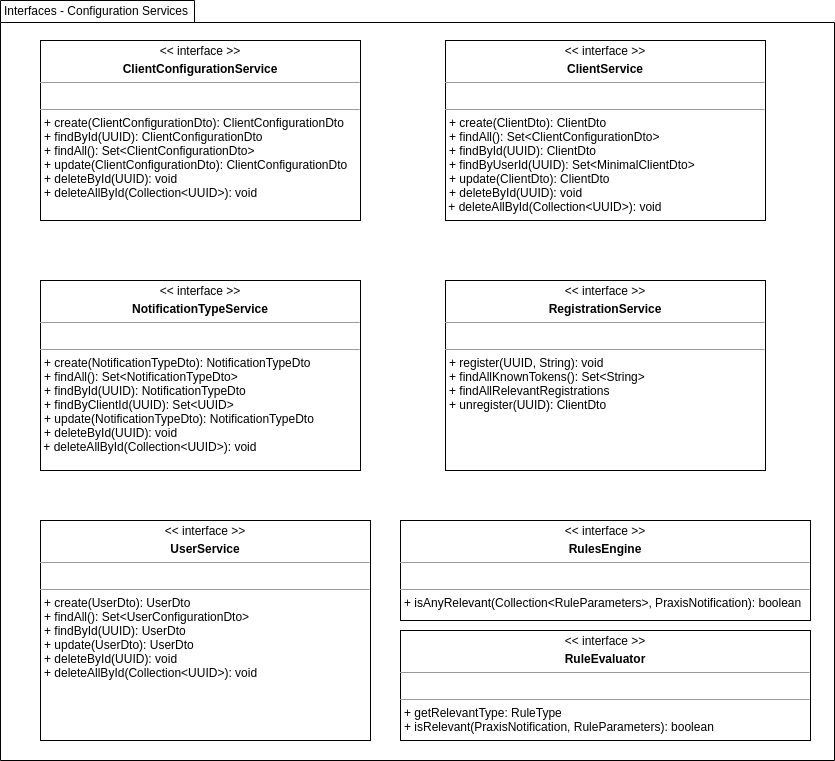
\includegraphics[width=\textwidth]{graphics/Class_Configuration_Services}
        \caption{Klassendiagramm Configuration Service Interfaces}
    \end{minipage}
\end{figure}

Abbildung 4.6 zeigt die Interfaces für Services welche es in der Configuration Domäne gibt.
ClientConfigurationService, ClientService, NotificationTypeService, RegistrationService und UserService bieten Create, Read, Update und Delete Methoden für das jeweilige Domänenobjekt an.
Diese Methoden sind zu Verwaltungszwecken über eine REST-API ansprechbar. Siehe Kapitel xy (API).

Der RegistrationService bietet dabei eine Ausnahme.
Der RegistrationService bietet Methoden um Registrierungen zu erfassen und wieder zu löschen.
Er bietet zudem die Möglichkeit anhand einer gegebenen Notification zu identifizieren, welche der registrierten Clients sich für diese Notification interessieren.
Diese Auswertungen werden mithilfe der RulesEngine gemacht.
Die RulesEngine bewertet die erfassten RulesParameter mithilfe der RuleEvaluators und findet alle relevanten tokens. Siehe Kapitel Rules Engine.

\clearpage
\subsubsection*{Rules Engine}


\begin{figure}[h]
    \centering
    \begin{minipage}[b]{0.9\textwidth}
        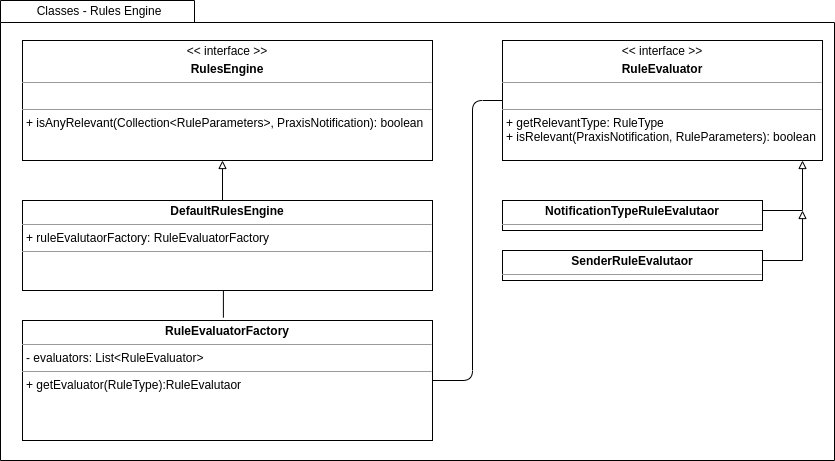
\includegraphics[width=\textwidth]{graphics/Class_Configuration_RulesEngine}
        \caption{Klassendiagramm Rules Engine}
    \end{minipage}
\end{figure}

Die RulesEngine ermöglicht es dem Cloud Service festzustellen, welche Benachrichtigungen an welche Clients versendet werden sollen.
Die RulesEngine selbst bietet dazu eine einzelne öffentliche Methode.
Diese nimmt eine Liste von Regelparametern (RulesParameters) und eine Notification entgegen.
Zurückgegeben wird ein Boolean wert, der sagt ob mindestens eine der übergebenen Regelparameter für die Benachrichtigung relevant ist.
Da jeder aktive Client eine ClientConfiguration definiert, die eine Liste an Regelparametern beinhaltet kann so mit der RulesEngine bewertet werden, ob ein bestimmter Client sich für eine Benachrichtigung interessiert.

Die Auswertung der einzelnen Regelparameter innerhalb der RulesEngine wird an einzelne RuleEvaluatoren delegiert.
Umgesetzt wird dieses Konzept mit einem Stragegy Pattern.
Wobei das RuleEvaluator Interface das Strategy Interface darstellt.
Der Zugriff auf die einzelnen Strategies innerhalb der RulesEngine wird über eine RuleEvaluatorFactory gelöst.
Diese Factory kennt alle existierenden RuleEvaluator Instanzen und bietet eine öffentliche Methode, über welche der RuleEvaluator für einen bestimmten Typ geladen werden kann.
Über die Dependency Injection des Spring Frameworks, kann diese RuleEvaluatorFactory einfach und erweiterbar implementiert werden:



\clearpage

\lstinputlisting[caption=RuleEvaluatorFactory.java,language=java,label={lst:RuleEvaluatorFactory.java}]{listings/RuleEvaluatorFactory.java}

Über den @Autowired Konstruktor nimmt die Factory eine Liste des Types RuleEvaluator entgegen.
Die Spring Dependency Injection wird hier automatisch alle verfügbaren RuleEvaluator Instanzen in einer Liste sammeln und als Konstruktorparameter entgegennehmen.
Da jeder RuleEvalutaor eine Methode bietet, über die der relevante RuleType abgefragt werden kann, kann nun aus dieser Liste eine Map gebaut werden, die RuleTypes auf die relevanten RuleEvaluator Instanzen mapped.
Das Laden eines RuleEvaluators ahnand des RuleTypes kann nun über ein einfaches Lookup in der Map erfolgen.
Werden in der Zukunft weitere RuleTypes unterstützt, reicht es die entsprechende RuleEvaluatorFactory zu implementieren.
Der neue RuleEvaluator wird danach automatisch über dei RuleEvaluatorFactory verfügbar sein.
Anpassungen an der RulesEngine oder der RuleEvaluatorFactory sind nicht nötig.


\clearpage
\subsubsection*{Domäne Notification}

Hier gehts darum Benachrichtigungen zu versenden.

\begin{figure}[h]
    \centering
    \begin{minipage}[b]{1.0\textwidth}
        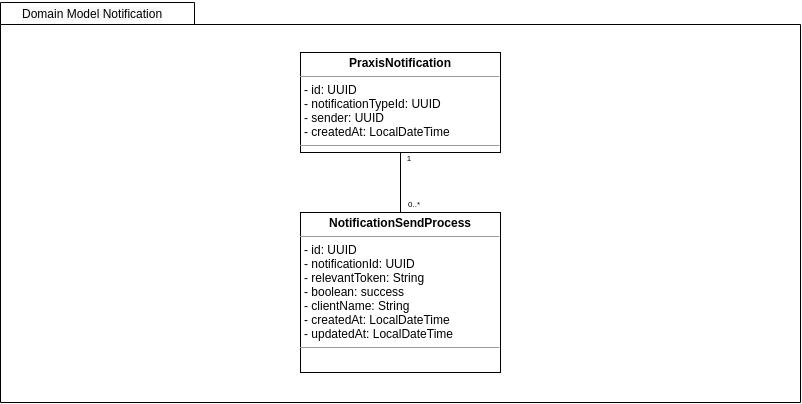
\includegraphics[width=\textwidth]{graphics/Class_Notification_Domain}
        \caption{Domänenmodell Notification}
    \end{minipage}
\end{figure}

\textbf{PraxisNotification}
Jede Notification die der CloudService erhält wird bereits vor dem Versenden persistiert.
Dient der Nachvollziehbarkeit.
Ermöglicht das Wiederholen von fehlgeschlagenen.

\textbf{SendNotificationProcess}
Für jeden Empfänger an den versucht wird eine Notification zu versenden, wird ein SendNotificationProcess erstellt.
Dient der Nachvollziehbarkeit.
Ermöglicht das Wiederholen von fehlgeschlagenen.

\clearpage

\subsubsection*{Services Notification}

\begin{figure}[h]
    \centering
    \begin{minipage}[b]{0.9\textwidth}
        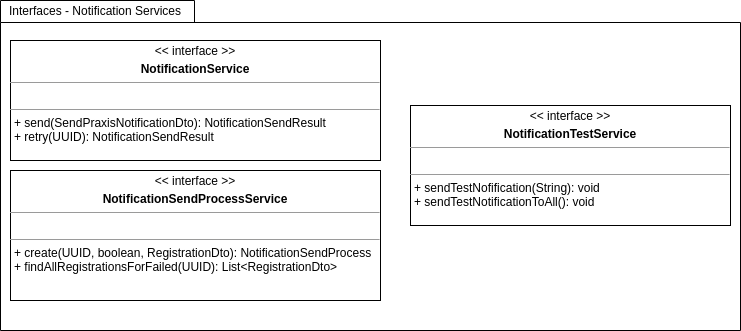
\includegraphics[width=\textwidth]{graphics/Class_Notification_Services}
        \caption{Klassendiagramm Notification Service Interfaces}
    \end{minipage}
\end{figure}


Der \textbf{NotificationService} bietet Methoden um eine Notifikation zu versenden und zu wiederholen.
Für das initiale Versenden werden die Informationen benötigt um eine Notifikation zu erstellen.
Im Fall der Wiederholung werden diese Informationen nicht mehr benötigt.
Da die Notifikation beim ersten Versuch sie zu versenden persistiert wurde.

Der \textbf{NotificationSendProcessService} dient dazu Sendevorgänge zu erstellen und fehlgeschlagene Sendevorgänge zu finden.
Dies ermöglicht es, eine Notifikation im Fehlerfall zu wiederholen.

Der \textbf{NotificationTestService} dient zu Test und Administrationszwecken.
Er kann verwendet werden um einem einzelnen Client eine Testnachricht zu senden oder allen Registrierten Clients eine Nachricht zu schicken.
Die Nachricht die hier versendet wird ist im Cloud Service vorgegeben.
Sie beinhaltet lediglich Platzhaltertexte und ist nicht konfigurierbar.

\clearpage
\subsubsection{Laufzeitmodell}

Im Folgenden werden die Abläufe für das Versenden und Empfangen von Benachrichtigungen im Detail definiert.

\subsubsection*{Client Registration}

Vorbedingung: Es wurde mindestens in Client inklusive ClientConfiguration erfasst und dem Praxismitarbeiter zugewiesen.

In einem ersten Schritt muss sich der Praxismitarbeiter am Mobile Client anmelden.
Hat er gültige Benutzerdaten angegeben, werden Informationen zu allen verfügbaren Konfigurationen vom Cloud Service geladen und der Benutzer kann die gewünschte Konfiguration auswählen.
Dabei werden nur Name und Id der Konfigurationen geladen, damit nicht mehr Daten als nötig übertragen werden.
Sobald eine Konfiguration ausgewählt ist, werden alle dafür Konfigurierten NotificationTypes geladen und im UI die entsprechenden Buttons erstellt.
Sobald eine Konfiguration geladen ist, registriert sich der Mobile Client beim Messageing Service.
Als Antwort erhält er ein eindeutiges Token, welches verwendet werden kann, um an diesem Client Nachrichten zu senden.
Der Mobile Client Registriert sich schliesslich mit dem Token vom Messaging Service und der ausgewählten Konfiguration beim Cloud Service.
In diesem Zustand ist der Client dem Messaging Service und dem Cloud Service bekannt und ist bereit Benachrichtigungen zu empfangen.

\begin{figure}[h]
    \centering
    \begin{minipage}[b]{0.9\textwidth}
        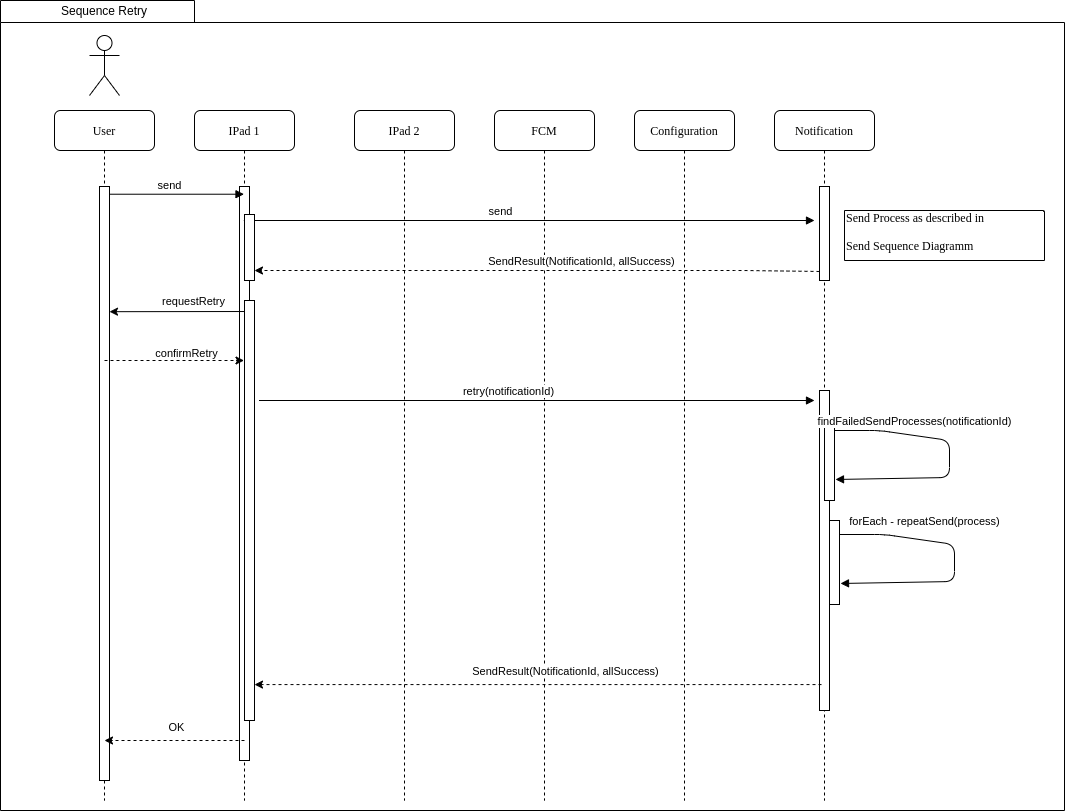
\includegraphics[width=\textwidth]{graphics/Sequence_Notification_Register}
        \caption{Ablauf Registration}
    \end{minipage}
\end{figure}


\subsubsection*{Benachrichtigung versenden und empfangen}

Pre-Condition: Client Registrierung ist für 2 Clients abgeschlossen. Es bestehen gültige Subscriber Configs. Konfiguration ist geladen.

Der Benutzer tippt auf einen der Benachrichtigungsbuttons.
Pro Button ist die Id des verbundenen NotificationTypes hinterlegt.
Es wird nun eine Anfrage an den NotificationController im Cloud Service gesendet.
Darin enthalten sind die Id des Absender Clients und die Id des NotificationTypes.
Der NotificationController macht eine Anfrage an den ConfigurationController um alle relevanten empfänger zu finden.
Im ConfigurationController werden alle konfigurierten ClientConfigurations nach Subscriber Regeln evaluiert.
Der ConfigurationController gibt schliesslich eine Liste der Registrations zurück die zu einer ClientConfiguration gehören für die eine der Konfigurierten Regeln zugetroffen hat.
Der NotificationController lädt den NotificationType aus der Send-Anfrage und benutzt diese Daten um eine Benachrichtigung an alle Empfänger für die er gerade Registrations geladen hat zu senden.
Der NotificationController meldet zurück, ob der Versand an alle Empfänger funktioniert hat.
Ist dies nicht der Fall wird der Retry-Process auf Client Seite gestartet.

\begin{figure}[h]
    \centering
    \begin{minipage}[b]{0.9\textwidth}
        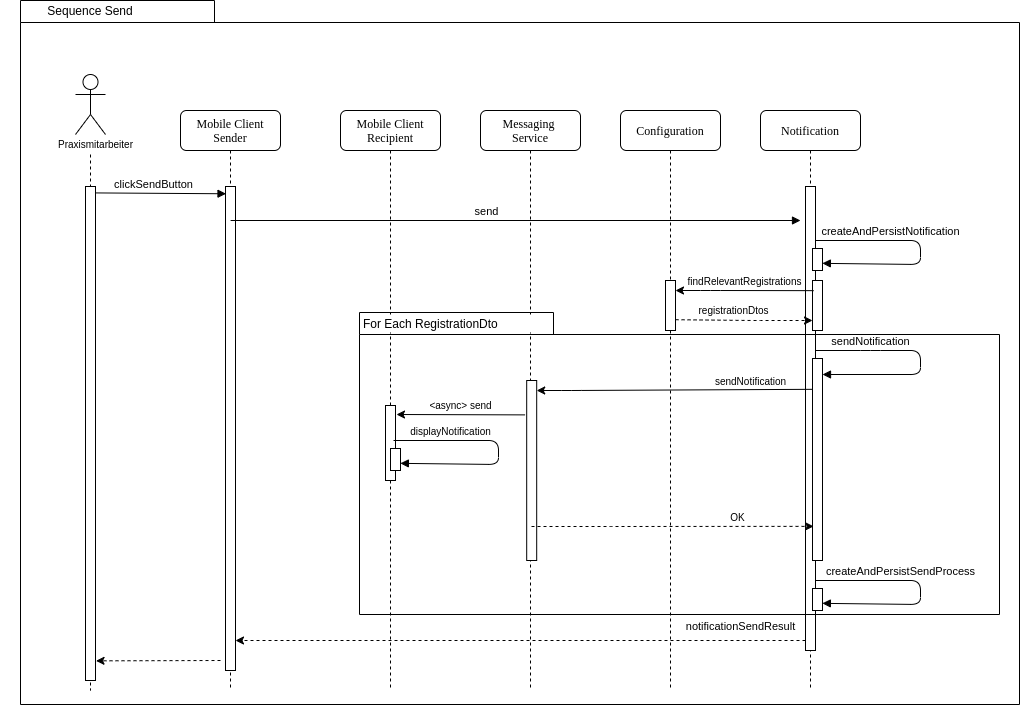
\includegraphics[width=\textwidth]{graphics/Sequence_Notification_Send}
        \caption{Ablauf Benachrichtigung Senden und Empfangen}
    \end{minipage}
\end{figure}


\clearpage
\subsubsection*{Benachrichtigung wiederholen}

\textbf{Vorbedingung:} Es wurde mindestens in Client inklusive ClientConfiguration erfasst und dem Praxismitarbeiter zugewiesen.
Es wurde ein zweiter Client inklusive ClientConfiguration erfasst.
Der zweite Client wurde so konfiguriert, dass er Benachrichtigungen die vom ersten Client empfängt.
Beide Clients laufen und haben sich bei Messaging Service sowie Cloud Service registriert.
Der Sender Client hat eine Benachrichtung versendet.
Das Versenden an mindestens einen Client aus dem Cloud Service ist fehlgeschlagen und der Cloud Service gibt ein negatives SendNotificationResult zurück.


Der Client zeigt einen Dialog an in dem der Benutzer informiert wird und gefragt wird, ob er die Fehlgeschlagenen wiederholen möchte.
Bestätigt der Benutzer wird eine Retry-Anfrage an den NotificationController gesendet.
Parameter ist die technische id der Notification die fehlgeschlagen ist.
NotificationController durchsucht die NotificationSendProcess tabelle nach der gegebenen id und filtert auf fehlgeschlagene.
Anschliessend wird der send prozess anhand der tokens in dieser NotificationSendProcess Instanzen wiederholt.

\begin{figure}[h]
    \centering
    \begin{minipage}[b]{0.9\textwidth}
        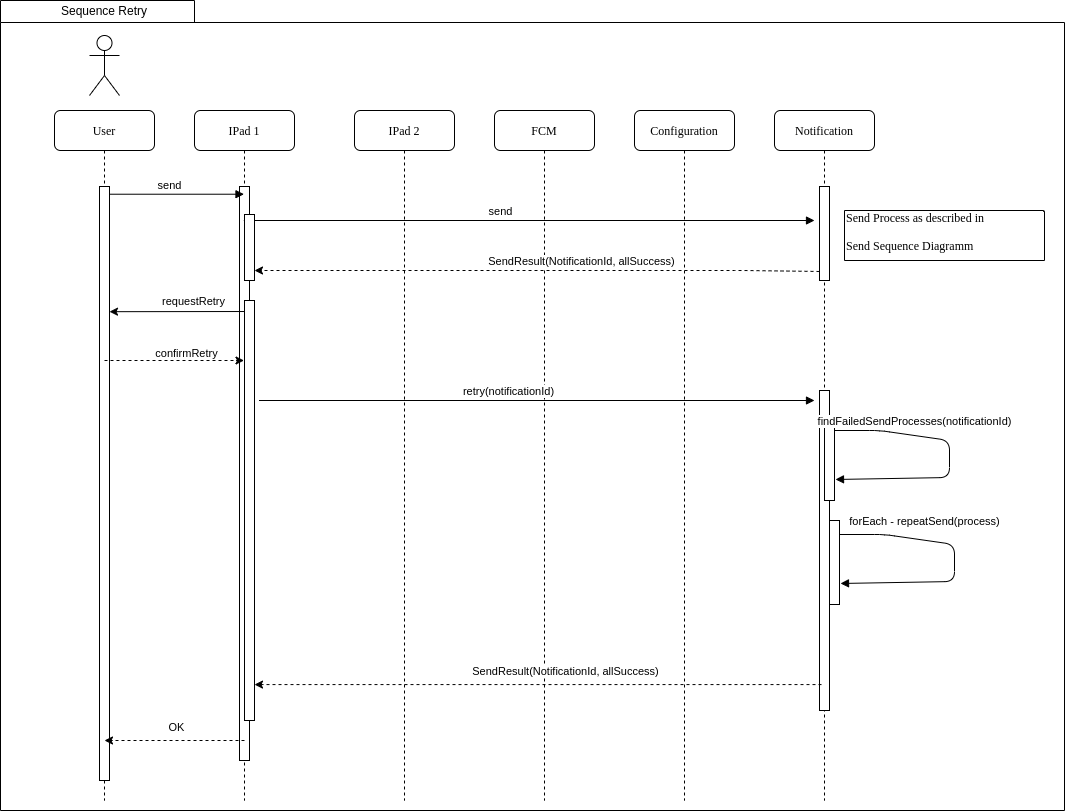
\includegraphics[width=\textwidth]{graphics/Sequence_Notification_Retry}
        \caption{Ablauf Benachrichtigung Wiederholen}
    \end{minipage}
\end{figure}


\clearpage

\subsubsection{API}

\subsubsection*{Verwaltung}

Um die Verwaltung der Konfigurationen zu ermöglichen, bietet der Cloud Service eine REST-API an über die Konfigurationsobjekte verwaltet werden können.
Der Cloud Service bietet Verwaltungs APIs für die Folgenden Domänenobjekte:

\begin{table}[h]
    \centering
    \begin{tabular}{|l|p{13cm}|}
        \hline
        \textbf{Domänenobjekt} & \textbf{Entity Name} \\
        \hline
        Client         & /api/clients \\
        \hline
        Client Configuration         & /api/client-configurations \\
        \hline
        Notification Types         & /api/notification-types \\
        \hline
        Users         & /api/users \\
        \hline
    \end{tabular}\label{tab:adminapimethods}
\end{table}

Für jedes dieser Domänenobjekte ist ein dedizierter Endpoint definiert, der unter dem Subpfad /api/entity-name erreichbar ist.
Jeder dieser Kontroller bietet eine API zu Verwaltung dieses Domänenobjekts, welche dem folgenden Schema folgt:

\begin{table}[h]
    \centering
    \begin{tabular}{|l|l|l|l|l|}
        \hline
        \textbf{Action} & \textbf{HTTP} & \textbf{Pfad} & \textbf{Body} & \textbf{Response} \\
        \hline
            Alle Elemente lesen         & GET & /api/entity-name & - & [EntityDto] \\
        \hline
            Einzelnes Element lesen         & GET & /api/entity-name/id & - & EntityDto \\
        \hline
            Neues Element erstellen         & POST & /api/entity-name  & EntityDto & EntityDto\\
        \hline
            Bestehendes Element ändern          & PUT & /api/entity-name  & EntityDto & EntityDto\\
        \hline
            Einzelnes Element löschen          & DELETE & /api/entity-name/id  & - & -  \\
        \hline
            Mehrere Elemente löschen          & DELETE & /api/entity-name/ids  & - & - \\
        \hline
    \end{tabular}\label{tab:apimethods}
\end{table}

Eine Ausnahme bildet hier das Domänenobjekt Registration.
Die Registrierung darf nie manuell von einem Administrator erfasst werden.
Sie muss immer von einem Mobile Client her kommen der sich beim Cloud Service registriert oder de-registriert.
Lesender Zugriff auf die Registrierungen ist nur nötig, wenn der Cloud Service eine Benachrichtigung versendet und die Messaging Tokens der relevanten Empfänger laden muss.
Dementsprechend bietet der RegistrationController nicht die volle Verwaltungs API sondern nur folgendes Subset:

\begin{table}[h]
    \centering
    \begin{tabular}{|l|l|l|l|l|}
        \hline
        \textbf{Aktion} & \textbf{HTTP} & \textbf{Pfad} & \textbf{Body} & \textbf{Response} \\
        \hline
        Registrierung aktualisiern         & POST & /api/registrations/ & ClientId, Messaging Token & - \\
        \hline
        Registrierung entfernen         & DELETE & /api/registrations/ & ClientId & - \\
        \hline
        Relevante Registrierung finden         & Post & /api/registrations/tokens & NotificationDto & [RegistrationDto] \\
        \hline
    \end{tabular}\label{tab:registrationsapimethods}
\end{table}

\clearpage

\subsubsection*{Fachliches}

Weiter gibt es Operationen welche eine fachliche Handlung darstellen die nicht der Verwaltung von Konfigurationen dienen.
Die API für diese Operationen folgen dem folgenden Schema:

/api/entity-name/action-name

Der Cloud Service bietet die folgenden fachlichen Endpunkte an:

\begin{table}[h]
    \centering
    \begin{tabular}{|l|l|l|l|l|}
        \hline
        \textbf{Aktion} & \textbf{HTTP} & \textbf{Pfad} & \textbf{Body} & \textbf{Response} \\
        \hline
        Notifikation versenden         & POST & /api/notifications/send & NotificationDto & NotificationSendResult \\
        \hline
        Notifikation wiederholen        & POST & /api/notifications/retry & Notification Id  & NotificationSendResult \\
        \hline
    \end{tabular}\label{tab:notificationapimethods}
\end{table}

\clearpage
